% The evaluation method (manuscript Section 4): inputs, one run, the studies under the two protocols, and the metrics.
% Build: pdflatex fig11_method.tex; pdftoppm -r 220 -png -singlefile fig11_method.pdf fig11_method
\documentclass[tikz,border=2pt]{standalone}
\usepackage{times}
\usetikzlibrary{positioning,arrows.meta,calc}
\begin{document}
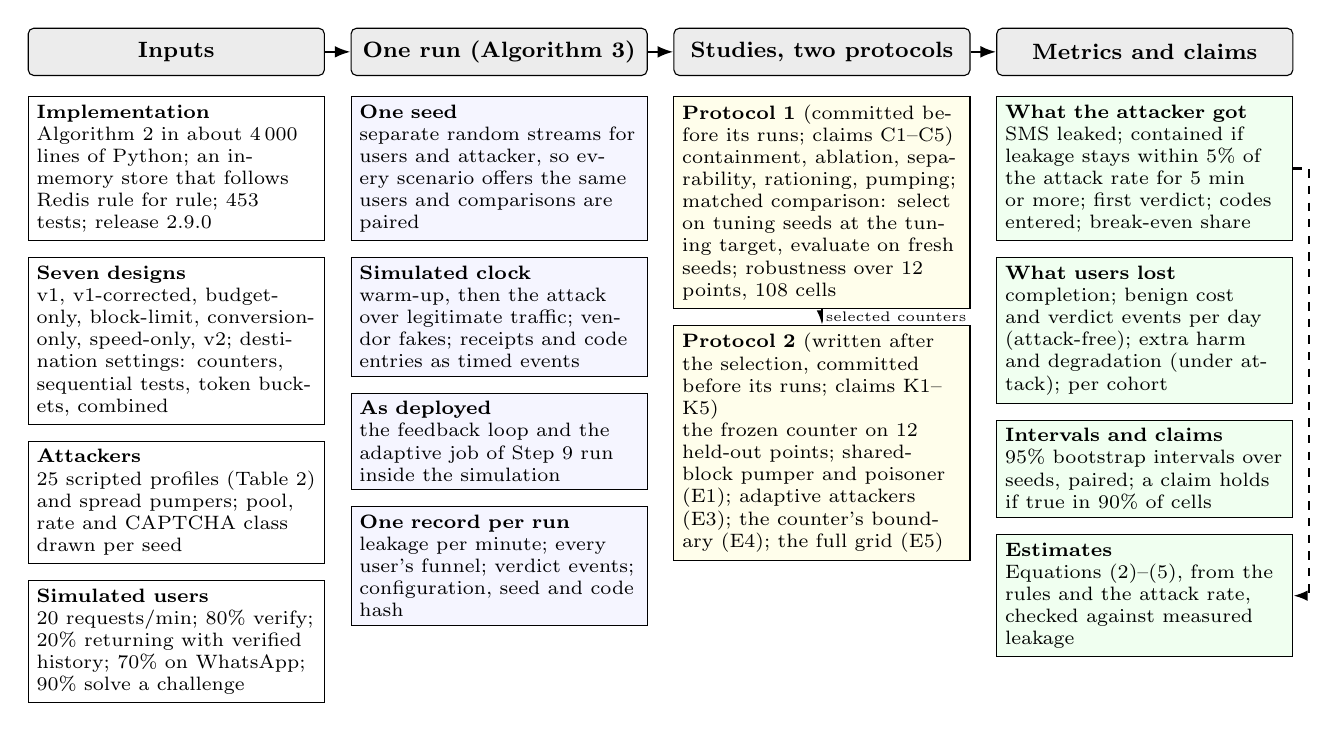
\begin{tikzpicture}[
  head/.style={draw, rounded corners=2pt, align=center, text width=3.55cm, minimum height=0.6cm, font=\footnotesize\bfseries, fill=gray!15, inner sep=3pt},
  box/.style={draw, align=left, text width=3.55cm, font=\scriptsize, inner sep=3pt, fill=white},
  proto/.style={box, fill=yellow!8},
  runbox/.style={box, fill=blue!4},
  metric/.style={box, fill=green!6},
  arr/.style={-{Latex[length=2mm]}, thick},
  ret/.style={-{Latex[length=1.8mm]}, thick, dashed},
  lab/.style={font=\tiny, fill=white, inner sep=1pt}
]
\def\dx{4.1cm}
% column headers
\node[head] (h1) at (0,0) {Inputs};
\node[head] (h2) at (\dx,0) {One run (Algorithm 3)};
\node[head] (h3) at (2*\dx,0) {Studies, two protocols};
\node[head] (h4) at (3*\dx,0) {Metrics and claims};

% column 1: inputs
\node[box, below=0.25cm of h1] (i1) {\textbf{Implementation}\\Algorithm 2 in about 4\,000 lines of Python; an in-memory store that follows Redis rule for rule; 453 tests; release 2.9.0};
\node[box, below=0.2cm of i1] (i2) {\textbf{Seven designs}\\v1, v1-corrected, budget-only, block-limit, conversion-only, speed-only, v2; destination settings: counters, sequential tests, token buckets, combined};
\node[box, below=0.2cm of i2] (i3) {\textbf{Attackers}\\25 scripted profiles (Table 2) and spread pumpers; pool, rate and CAPTCHA class drawn per seed};
\node[box, below=0.2cm of i3] (i4) {\textbf{Simulated users}\\20 requests/min; 80\% verify; 20\% returning with verified history; 70\% on WhatsApp; 90\% solve a challenge};

% column 2: one run
\node[runbox, below=0.25cm of h2] (r1) {\textbf{One seed}\\separate random streams for users and attacker, so every scenario offers the same users and comparisons are paired};
\node[runbox, below=0.2cm of r1] (r2) {\textbf{Simulated clock}\\warm-up, then the attack over legitimate traffic; vendor fakes; receipts and code entries as timed events};
\node[runbox, below=0.2cm of r2] (r3) {\textbf{As deployed}\\the feedback loop and the adaptive job of Step 9 run inside the simulation};
\node[runbox, below=0.2cm of r3] (r4) {\textbf{One record per run}\\leakage per minute; every user's funnel; verdict events; configuration, seed and code hash};

% column 3: studies
\node[proto, below=0.25cm of h3] (p1) {\textbf{Protocol 1} (committed before its runs; claims C1--C5)\\containment, ablation, separability, rationing, pumping; matched comparison: select on tuning seeds at the tuning target, evaluate on fresh seeds; robustness over 12 points, 108 cells};
\node[proto, below=0.2cm of p1] (p2) {\textbf{Protocol 2} (written after the selection, committed before its runs; claims K1--K5)\\the frozen counter on 12 held-out points; shared-block pumper and poisoner (E1); adaptive attackers (E3); the counter's boundary (E4); the full grid (E5)};

% column 4: metrics
\node[metric, below=0.25cm of h4] (m1) {\textbf{What the attacker got}\\SMS leaked; contained if leakage stays within 5\% of the attack rate for 5 min or more; first verdict; codes entered; break-even share};
\node[metric, below=0.2cm of m1] (m2) {\textbf{What users lost}\\completion; benign cost and verdict events per day (attack-free); extra harm and degradation (under attack); per cohort};
\node[metric, below=0.2cm of m2] (m4) {\textbf{Intervals and claims}\\95\% bootstrap intervals over seeds, paired; a claim holds if true in 90\% of cells};
\node[metric, below=0.2cm of m4] (m5) {\textbf{Estimates}\\Equations (2)--(5), from the rules and the attack rate, checked against measured leakage};

% flow between columns
\draw[arr] (h1) -- (h2); \draw[arr] (h2) -- (h3); \draw[arr] (h3) -- (h4);
% the selection feeds the second protocol
\draw[ret] (p1.south) -- node[lab, right]{selected counters} (p2.north);
% the estimates are checked against measured leakage
\draw[ret] (m1.east) -- ++(0.2,0) |- (m5.east);
\end{tikzpicture}
\end{document}
